\section{Account structure}\label{sec:account}

An account is composed by a set of attributes, represented by an address, managed by a set of private keys and incorporates a set of functionalities. These functionalities include spending money that are held by the account and taking part in Proof-of-Stake protocol-related actions. An account consists of multiple attributes that pertain to and are used on different functionalities and are organized in a tree, the root of which is the core identifier of the account.
 
DEFINE ATTRIBUTES.  $T_1, T_2, \ldots, T_m$

$f: T_1 \times \ldots \times T_m \rightarrow A$.

\subsection{Definitions}

\begin{defn}[Account keyset]\label{def:keyset}
The account key pair $K$ is a tuple of two keys, the payment key $K^p$ and the staking key $K^s$.
\end{defn}

$K^p$ is used for payment transactions, i.e. transferring the coins that are held by the account to a different account. $K^s$ is used for taking part in the Proof-of-Stake protocol, either as a committee member or a slot leader. $K^s$ can be also used for delegating the stake to a different staking key.

\begin{defn}[Account address]\label{def:address}
The address of an account is a string $\alpha \in \{0, 1\}^\mu$.
\end{defn}

$\alpha$ is a string that represents an account and can be used to extract information about it. Such information might be public or might be used in conjuction with other data in order to verify the actions that the owner of the account takes. A primary example of such data is the hash of the payment key. This hash is used when creating the address and it becomes public when the balance is spent. An account's address must correspond to all attributes of the account, so that a claim that an attribute is part of the account can be proved by providing a proof that it is linked to the account's address.

For the rest of the paper we will use the address $\alpha$ to describe the account that is identified by $\alpha$.

\begin{defn}[Address generation function]\label{def:addressgen}
The address generation function $f(\cdot)$ is a function that takes as parameters a set of account attributes $T$ and outputs an address $\alpha$.
\end{defn}

The implementation of $f$ and the objects in $T$ depend on the specifications of the protocol. $T$ may contain data like the keyset, the index of the keyset in the context of a hierarchical wallet generation etc.


\begin{defn}[Hierarchical wallet tag]\label{def:hierarchical_tag}
The hierarchical wallet tag $ht$ is a tag that is used to identify whether an address is part of a hierarchical wallet structure.
\end{defn}

\subsection{Account attributes}

The account's attributes are the moving parts that define an individual account. All of these parts must be used to create the account's address, so that, given two addresses $\alpha, \alpha'$ where $\alpha = \alpha'$ then $T = T'$, where $T, T'$ are the attribute sets for the two accounts respectively.

\begin{defn}[Spending set]\label{def:spending_part}
The spending set $S$ of an account is a set of attributes that are revealed when a transaction is created that spends from the account. The hash of the spending set is $H_s$.
\end{defn}

We include all attributes in the spending part of the tree to avoid a spending malleability attack. In such scenario, an attacker $A$ wishes to send some money to an honest receiver $B$, so she obtains an address $\alpha$ from $B$. She is successful if she is able to change $\alpha$ and create and address $\alpha'$, so that the balance in $\alpha'$ can be spent using the same payment key that was used to create $\alpha$, whilst some other attribute of $\alpha$, e.g. the staking key, has been replaced with an adversarial one.

\subsubsection{Public attributes}

Public attributes are attributes that need be publicly visible in the address. Specifically, they must exist in plaintext form in the address and can be recognized and used by the system automatically in order to complete protocol-related functionalities.

A public attribute is present in both the address and the spending set $S$.

Examples of public attributes are the delegation pointer, in case of an pointer account, or the hierarchical wallet tag.

\subsubsection{Private attributes}

These attributes become public only when a transaction is published that spends the entire account's balance.

Private attributes are present only in the spending set $S$ and are revealed only when a spending transaction is made.

The primary example of such an attribute is the payment key $K^p$.

\subsubsection{Hanging attributes}

Hanging attributes are not public by default, but may become public ahead of spending. Specifically, a hanging attribute might be used in protocol-related functions that are completed by the user and not by the system automatically.

A hanging attribute exists in both the spending set $S$ and a branch in the tree that defines the account. Specifically, the root of the tree that defines the account is the result of hashing $H_s$ with the hashes of all hanging attributes of the account.

An example of such attribute is the staking key $K^s$.

\subsection{Address structure}

The address of an account is the concatenation of the root of the tree that identifies the account with the public attributes of the account.

We now describe the structure of the address of three types of accounts, the \textbf{base} account, the \textbf{pointer} account and the \textbf{exchange} account. These types of accounts differ on the way the stake that they hold is delegated, as well as the structure of the address that represents them.

\subsubsection{Base account}\label{subsubsec:base_account_v2}

A base account is managed by the payment key $K^p$. This account is formed by this key along with the public attributes that are the hash of a staking key $K^s$, which we call delegation hash $dh$, and the hierarchical tag $ht$.

The core part of the address is the root of the attribute tree. This is the hash of all attributes in the spending set, i.e. the payment key and the public attributes.

The stake that is held by the base account is delegated to the staking key $K^s$. Therefore the account links to the staking information, which is in this case the staking key.

The attributes and the address structure of a base account can be seen in Figure \ref{fig:base_account_v2}.

\begin{figure}
  \begin{center}
    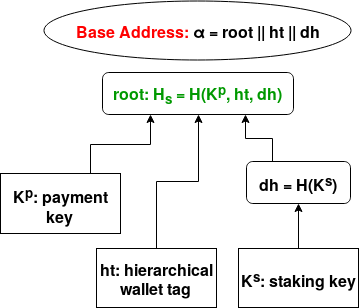
\includegraphics[width=230pt]{base_account_v2.png}
  \end{center}
  \caption{The base account.}
  \label{fig:base_account_v2}
\end{figure}

\subsubsection{Pointer account}\label{subsubsec:pointer_account}

A pointer account is managed by a single payment key $K^p$. Therefore, the owner of such account can only complete one action, that is spending the balance of the account, whereas all other actions that pertain to the Proof-of-Stake protocol are completed by the system.

The core part of the address is again the root of the attribute tree. However, in this case this part is just the hash of all of the account's attributes, i.e. it is the hash of the spending set defined in \ref{def:spending_part}. The rest of the address consists of the hierarchical wallet tag and the delegation pointer.

The delegation pointer is used to identify the staking key that the stake in the account is delegated to. Specifically, the pointer points to a transaction that contains a registration certificate for a staking key that has been published on the blockchain. That way the delegate key for the pointer address is the one defined in the certificate that the account points to and, given that this information is included in the address in plaintext form, the stake in the pointer account is delegated to the registered staking key. Similarly to the base account described above, the pointer account links to the staking information.

The attributes and the address structure of a pointer account can be seen in Figure \ref{fig:pointer_account}.

\begin{figure}
  \begin{center}
    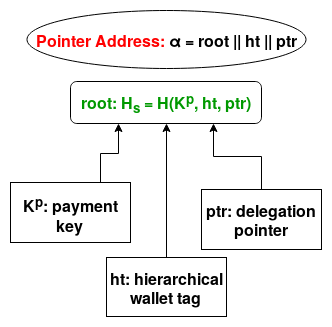
\includegraphics[width=210pt]{pointer_account.png}
  \end{center}
  \caption{The pointer account.}
  \label{fig:pointer_account}
\end{figure}

\subsubsection{Enterprise account}\label{subsubsec:exchange_account_plain}

An exchange account is an account managed by a payment key $K^p$. The stake in this account is not delegated to any staking key and is excluded from all protocol operations, like the block creation. An exchange account is identified by the exchange identifier $\epsilon$, which is a public attribute of the account.

The address structure of an exchange account can be seen in Figure \ref{fig:exchange_account_plain}.

\begin{figure}
  \begin{center}
    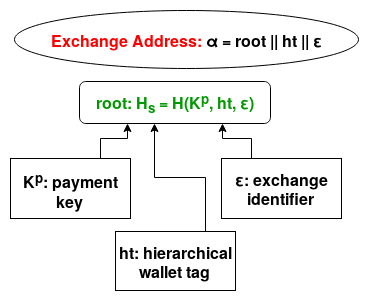
\includegraphics[width=210pt]{exchange_account_plain.png}
  \end{center}
  \caption{The exchange account.}
  \label{fig:exchange_account_plain}
\end{figure}